\documentclass[a4paper,14pt]{extarticle}

\usepackage[utf8x]{inputenc}
\usepackage[T1,T2A]{fontenc}
\usepackage[russian]{babel}
\usepackage{hyperref}
\usepackage{indentfirst}
\usepackage{here}
\usepackage{array}
\usepackage[table]{xcolor}
\usepackage{datetime}
\usepackage{multirow}
\usepackage{hhline}
\usepackage{mathtools,cancel}
\usepackage{forest}
\usepackage{graphicx}
\usepackage{caption}
\usepackage{subcaption}
\usepackage{chngcntr}
\usepackage{amsmath}
\usepackage{amssymb}
\usepackage{pgfplots}
\usepackage{pgfplotstable}
\usepackage[left=2cm,right=2cm,top=2cm,bottom=2cm,bindingoffset=0cm]{geometry}
\usepackage{multicol}
\usepackage{askmaps}
\usepackage{tikz}

\newcommand*\circled[1]{\tikz[baseline=(char.base)]{
            \node[shape=circle,draw,inner sep=2pt] (char) {#1};}}

\DeclareMathOperator*{\argmin}{argmin}

\renewcommand{\not}[1]{\mkern 1.5mu\overline{\mkern-1.5mu#1\mkern-1.5mu}\mkern 1.5mu}
\renewcommand{\le}{\ensuremath{\leqslant}}
\renewcommand{\leq}{\ensuremath{\leqslant}}
\renewcommand{\ge}{\ensuremath{\geqslant}}
\renewcommand{\geq}{\ensuremath{\geqslant}}
\renewcommand{\epsilon}{\ensuremath{\varepsilon}}
\renewcommand{\phi}{\ensuremath{\varphi}}

\counterwithin{figure}{section}
\counterwithin{equation}{section}
\counterwithin{table}{section}
\newcommand{\sign}[1][5cm]{\makebox[#1]{\hrulefill}} % Поля подписи и даты
\graphicspath{{pics/}} % Путь до папки с картинками
\captionsetup{justification=centering,margin=1cm}
\def\arraystretch{1.3}

\begin{document}

\begin{titlepage}
\begin{center}
	Санкт-Петербургский политехнический университет Петра Великого\\[0.3cm]
	Институт компьютерных наук и технологий \\[0.3cm]
	Кафедра компьютерных систем и программных технологий\\[4cm]
	
	\textbf{Расчётное задание №6}\\[2mm]
	\textbf{Дисциплина:} Системный анализ и принятие решений\\[2mm]
	\textbf{Тема:} Дискретное программирование. Задача коммивояжёра\\[2mm]
	Вариант 39\\[6.5cm]
\end{center}

\begin{flushleft}
	\hspace*{5mm} Выполнил студент гр. 33501/4  \hspace*{3cm}\sign[3cm]\hspace*{2mm} А.Ю. Ламтев\\
	\hspace*{10.85cm} (подпись)\\[2.5mm]
	\hspace*{5mm} Преподаватель \hspace*{6.45cm}\sign[3cm]\hspace*{2mm} С.С. Сабонис\\
	\hspace*{10.85cm} (подпись)\\[2.5mm]
	\hspace*{11.1cm} <<\underline{\the\day}>> \underline{\hspace{5mm}ноября\hspace{5mm}} \the\year\hspace{1mm} г.
\end{flushleft}

\vfill

\begin{center}
	Санкт-Петербург\\
	\the\year
\end{center}
\end{titlepage}
\addtocounter{page}{1}

\section{Задание}

Сравнить средние времена пребывания и средние времена ожидания для разных систем в зависимости от интенсивности потока заявок.  Построить соответствующие графики.  Какая система лучше (при каких интенсивностях первая система лучше, при каких – вторая)? 

Исходные данные:\\

На рис. \ref{pic:mm44} -- \ref{pic:mm14} представлены сравниваемые СМО.

\begin{figure}[H]
	\begin{center}
		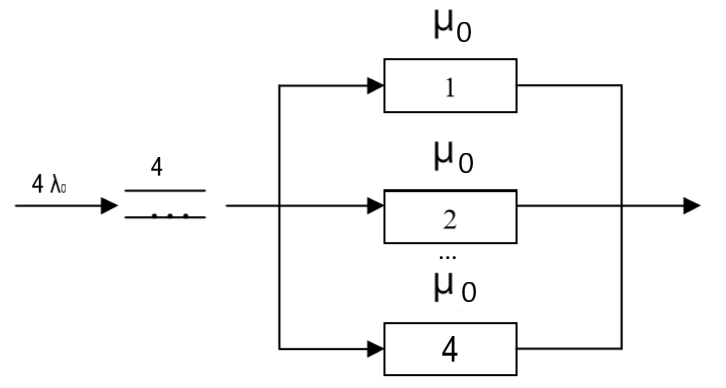
\includegraphics[width=\textwidth]{mm44}
		\caption{СМО $M/M/4/4$}
		\label{pic:mm44}
	\end{center}
\end{figure}

\begin{figure}[H]
	\begin{center}
		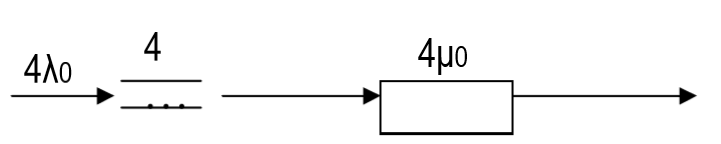
\includegraphics[width=\textwidth]{mm14}
		\caption{СМО $M/M/1/4$}
		\label{pic:mm14}
	\end{center}
\end{figure}

\section{Расчет многоканальной СМО с ограниченной очередью}

C помощью \verb+Python+ выполним расчет СМО по следующим формулам:

\begin{itemize}
	\item Суммарный коэфициент загрузки в системе \begin{equation*}
		\rho_c = \frac{\lambda}{K \cdot \mu}
	\end{equation*}
	\item Вероятность простоя системы \begin{equation*}
		P_0 = \left[ 1 + \sum_{j = 1}^4 \frac{\rho^j}{j!} + \frac{\rho^5 (1 - (\frac{\lambda}{\mu})^4)}{4!(1 - \frac{\lambda}{\mu}) \cdot 4} \right]^{-1}
	\end{equation*}
	\item Вероятность отказа в обслуживании \begin{equation*}
		P_\text{отк} = \frac{\rho^{K + m} P_0}{K^mK!}
	\end{equation*}
	\item Среднее число требований в очереди \begin{equation*}
		\not{n_0} = \frac{\rho^{K+1}P_0(1 - \rho_c^m(m + 1 - m\rho_c))}{K(1-\rho_c)^2K!}
	\end{equation*}
	\item Среднее время ожидания требования в очереди \begin{equation*}
		\not{t_\text{ож}} = \frac{\not{n_0}}{\rho \cdot \mu}
	\end{equation*}
	\item Среднее время пребывания требования в системе \begin{equation*}
		\not{t_\text{c}} = \not{t_\text{ож}} + \frac{1}{\mu}(1 - P_\text{отк})
	\end{equation*}
\end{itemize}

\section{Расчет одноканальной СМО с ограниченной очередью}

C помощью \verb+Python+ выполним расчет СМО по следующим формулам:

\begin{itemize}
	\item Среднее время ожидания требования в очереди \begin{equation*}
		\not{t_\text{ож}} = \frac{\rho (1-\rho^m(1+m-mp))}{\mu (1-\rho)(1-\rho^{m+2})}
	\end{equation*}
	\item Среднее время пребывания требования в системе \begin{equation*}
		\not{t_\text{c}} = \frac{(1-\rho^{m+1}(2+m-\rho-m\rho))}{\mu(1-\rho)(1-\rho^{m+2})}
	\end{equation*}
\end{itemize}

\section{Сравнение СМО}

Построим графики зависимостей $\not{t_\text{ож}} = f(\lambda)$ и $\not{t_\text{c}} = f(\lambda)$ для двух СМО на интервале $\rho \in (0,\ 1)$ для СМО $M/M/1/4$ и на интервале $\rho_c \in (0,\ 1)$ для СМО $M/M/4/4$. На выбранных интервалах системы являются устойчивыми, т.е. имеют конечные средние задержки и длины очереди.

\begin{figure}[H]
	\begin{center}
		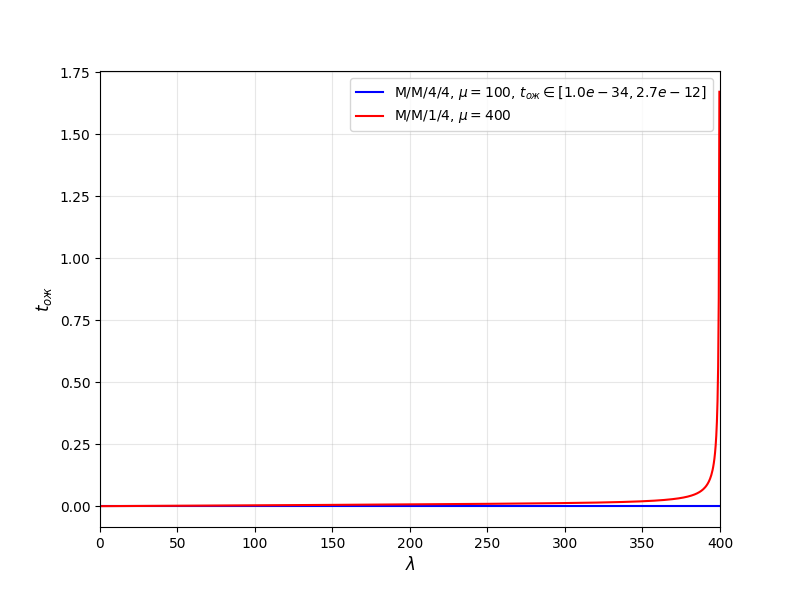
\includegraphics[width=\textwidth]{to}
		\caption{$\not{t_\text{ож}} = f(\lambda)$}
		\label{pic:to}
	\end{center}
\end{figure}

\begin{figure}[H]
	\begin{center}
		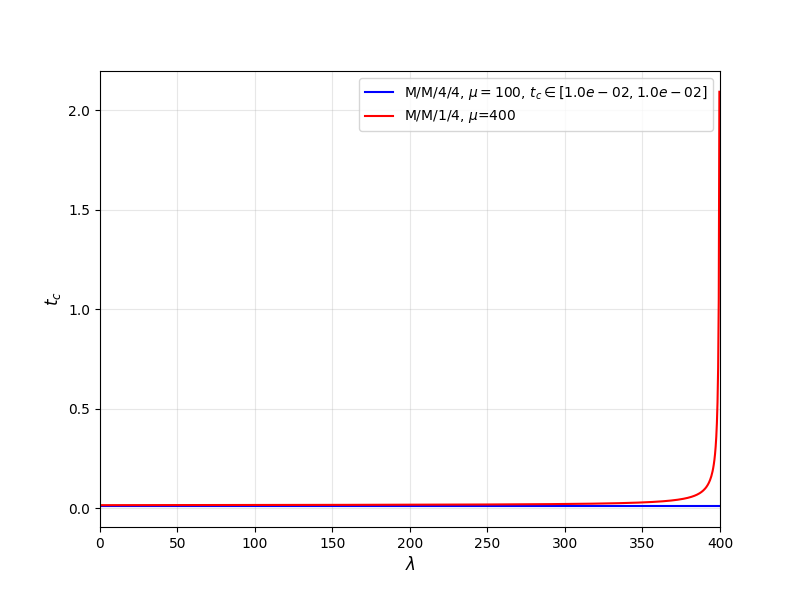
\includegraphics[width=\textwidth]{tc}
		\caption{$\not{t_\text{c}} = f(\lambda)$}
		\label{pic:tc}
	\end{center}
\end{figure}

На рис. \ref{pic:to} -- \ref{pic:tc} видно, что среднее время ожидания требования в очереди и среднее время пребывания требования в системе для СМО $M/M/1/4$ растут быстрее, чем для СМО $M/M/4/4$. Таким образом, $M/M/4/4$ лучше, чем $M/M/1/4$ по временным показателям для интенсивностей $\lambda \in (0,\ 4\mu_0]$

\end{document}